\documentclass[12pt]{../../../notes}
\usepackage{silence}
\WarningFilter{latex}{Reference}
\graphicspath{{../../img/}}

\begin{document}

\paragraph{Матрицы, основные определения}
\begin{defn}[Матрицы над $K$]\label{defn:matrices}
  Пусть $K$"--- поле, $m,n\in \N$. Тогда
  \[
    M_{m,n}(K) = 
    \left\{
      A 
    \,\middle|\,
      A  = 
      \begin{pmatrix}
        a_{11} & a_{12} & \cdots & a_{1n} \\
        a_{11} & a_{12} & \cdots & a_{1n} \\
        \vdots & \vdots & \ddots & \vdots \\
        a_{m1} & a_{m2} & \cdots & a_{mb}
      \end{pmatrix},\;
      a_{ij} \in K
    \right\}
  \]
\end{defn}

\begin{defn}[Сложение матриц]\label{defn:matradd}
  $A_{mn}\cdot B_{mn}:$
  \[
    (a+b)_{ij} = a_{ij} + b_{ij}
  \]
\end{defn}

\begin{defn}[Умножение матриц]\label{defn:matrmul}
  $A_{mn}\cdot B_{nk}:$
  \[
    (ab)_{ij} = \sum_{l=1}^n a_{i\ell}\cdot b_{\ell j}
  \]
\end{defn}

\paragraph{Кольцо квадратных матриц}
Обозначается $M_n(K)$

\noindent Ноль:
\[
  Z_n = 
  \begin{pmatrix}
    0      & 0      & \cdots & 0 \\
    0      & 0      & \cdots & 0 \\
    \vdots & \vdots & \ddots & \vdots \\
    0      & 0      & \cdots & 0 \\
  \end{pmatrix}
\]
Единица:
\[
  E_n = 
  \begin{pmatrix}
    1      & 0      & \cdots & 0 \\
    0      & 1      & \cdots & 0 \\
    \vdots & \vdots & \ddots & \vdots \\
    0      & 0      & \cdots & 1 \\
  \end{pmatrix}
\]
\parrange{2}{Определитель}
\begin{defn}\label{defn:determinant}
  Пусть $A\in M_n(K)$
  \[
    \det A = \sum_{\sigma \in S_n} (-1)^{I(\sigma)} \cdot a_{1\sigma(1)} \dotsm a_{n\sigma(n)}
  \]
\end{defn}
\begin{defn}\label{defn:determrows}
  Если обозначать строки $A_1, \dotsc , A_n$, а столбцы $A^{(1)}, \dotsc , A^{(n)}$,
  то можно ввести ещё такую функцию:
  \[
    \det (A_1, \dotsc , A_n) = \det (A^{(1)}, \dotsc , A^{(n)}) := \det A
  \]
\end{defn}

\begin{defn}[Элементарные преобразования]\label{defn:elemtranf}
  \noindent\newline\par
  \begin{tabular}{c|l|l}
    I   & $A_i \leftrightarrows A_j$ & $A^{(i)} \leftrightarrows A^{(j)}$     \\
    II  & $A_i := A_i + \lambda A_j$ & $A^{(i)} := A^{(i)} + \lambda A^{(j)}$ \\
    III & $A_i := \lambda A_i$       & $A^{(i)} := \lambda A^{(i)}$           
  \end{tabular}
\end{defn}
\begin{defn}[Транспонированная матрица]\label{defn:transpose}
  \[
    A^T \colon (a^T)_{ij} = (a)_{ij}
  \]
\end{defn}

\subparagraph{Свойства}
\begin{enumerate}
  \item Определитель (в описанном в~\ref{defn:determrows} смысле) полилинеен и кососимметричен по
    строкам и столбцам.
  \item Если 2 строчки или столбца одинаковые, то определитель равен 0
  \item Элементарные преобразования влияют на определитель следующим образом:\par
    \begin{tabular}{c|r}
      I   & $(-1)\det A$ \\
      II  & $\det A$     \\
      III & $\lambda \det A$
    \end{tabular}
  \item $\det A^T = \det A$
\end{enumerate}


\paragraph{Теорема Лапласа}
\begin{defn}[Минор]\label{defn:minor}
  Пусть $A\in M_n(K)$, а $k\in \N$. Тогда определитель подматрицы, собранной из $k$ строк и $k$
  столбцов называется \emph{минором} порядка $k$.
  \[
    \Delta = 
    \begin{vmatrix}
      a_{i_1j_1} & \cdots & a_{i_1j_k} \\
      \vdots & \ddots & \vdots \\
      a_{i_kj_1} & \cdots & a_{i_kj_k} 
    \end{vmatrix}
  \]
  $\Delta'$~--- дополнительный минор"--- всё, что осталось.
  Его ещё иногда (когда минор"--- один элемент) обозначают как $M_{ij}$
\end{defn}
\begin{defn}[Алгебраическое дополнение]\label{defn:cofactor}
  \[
    A_\Delta = (-1)^{i_1 + \dotsb + i_k + j_1 + \dotsb + j_k} \Delta'
  \]
\end{defn}

\begin{thrm}[Теорема Лапласа]\label{thrm:laplacecofactor}
  Пусть $A\in M_n(K)$, $k\in \N$. Выберем из матрицы $k$ строчек. Тогда
  \[
    \det A = \sum_{\Delta} \Delta \cdot A_\Delta
  \]
  где $\Delta$~--- любой минор, содержащий нужные $k$ строчек.
\end{thrm}
\begin{ittproof}
  Выберем какой-то один минор, $i_k$~--- его строчки, $j_\ell$~--- его столбцы
  \[
    \Delta : 
    \begin{cases}
      i_1, \dotsc , i_k \\
      j_1, \dotsc , j_k
    \end{cases}
  \]
  Теперь отправим все элементы, попавшие в минор, в левый верхний угол.
  Сначала сдвинем все строчки:
  \[
    \begin{cases}
      i_1 \to 1 & (i_1 -1 \text{~сдвигов})\\
      \hdotsfor{2} \\
      i_k \to k & (i_k - k \text{~сдвигов})
    \end{cases}
  \]
  Потом все столбцы
  \[
    \begin{cases}
      j_1 \to 1 & (i_1 - 1 \text{~сдвигов})\\
      \hdotsfor{2} \\
      j_k \to k & (i_k - k \text{~сдвигов})
    \end{cases}
  \]
  В итоге, из свойств элементарных преобразований, получим: 
  \[
    \det B = (-1)^{i_1 - 1 + \dotsb + i_k - k + j_1 - 1 + \dotsb + j_k - k} \det A 
    = (-1)^{i_1  + \dotsb + i_k  + j_1  + \dotsb + j_k } \det A 
  \]
  так как все добавки парные $\Rightarrow$ делится на $2$.

  С другой стороны, $\Delta$ и $\Delta'$ никак не поменялись, так как переставляемые чиселки в
  них не не входят. Также нужно отметить, что $B_\Delta = \Delta'$, по тем же причинам, в
  общем-то.

  Посмотрим, что такое  $\Delta\cdot \Delta'$
  \footnote{Вообще, тут маленькая неточность: здесь фактически 
      \emph{действие} группы перестановок на множестве $\{k+1, \dotsc , n\}$}.
  \begin{align*}
    \Delta \cdot \Delta' 
    &= \Bigg( \sum_{\tau \in S_k} (-1)^{I(\tau)} b_{1\tau(1)} \dotsm
    b_{k\tau(k)} \Bigg) \cdot \Bigg( \sum_{\tau' \in S_{n-k}} (-1)^{I(\tau')} b_{k+1\tau'(k+1)} \dotsm
    b_{n\tau(n)} \Bigg)
  \end{align*}
  Пусть теперь $\sigma = \tau \circ \tau'$. Тогда $I(\sigma) = I(\tau)+I(\tau')$ по свойствам
  перестановок, а $\sigma$ фактически разбивается на 2 независимых цикла: $\tau$ и $\tau'$.
  В итоге
  \[
    \Delta \cdot \Delta' 
    = \sum_{\sigma\in S_n} (-1)^{I(\sigma)} b_{1\sigma(1)} \dotsm b_{n\sigma(n)}
  \]
  А это вообще-то правильный кусок определителя $B$. 
  Поймём, что это за кусок определителя $A$.
  Числа-то те же самые. А вот на вопрос со знаком мы уже по сути ответили, когда рассуждали про 
  определитель. Слагаемые точно не перемешиваются, так что каждое слагаемое просто умножается на
  $(-1){\cdots}$. 
  Так что 
  \begin{align*}
    \Delta \cdot \Delta' &= (-1)^{i_1  + \dotsb + i_k  + j_1  + \dotsb + j_k } 
    \sum_{\sigma'} a_{1\sigma'(1)} \dotsm a_{n\sigma'(n)} \\
    A_{\Delta} &= (-1)^{i_1  + \dotsb + i_k  + j_1  + \dotsb + j_k } \Delta'  \\
    \Delta \cdot A_{\Delta} &= \sum_{\sigma'} a_{1\sigma'(1)} \dotsm a_{n\sigma'(n)}
  \end{align*}
  где у $\sigma'$ уже другие независимые циклы: ${i_1, \dotsc , i_k\choose j_1, \dotsc , j_k }$ 
  и всё остальное.

\end{ittproof}
\begin{imp}
  \[
    \det A = a_{i1} A_{i1} + \dotsb + a_{in} A_{in} 
  \]
\end{imp}
\begin{imp}
  \[
    a_{j1} A_{i1} + \dotsb + a_{jn} A_{in} = 0
  \]
\end{imp}
\begin{itlproof}
  Приравняем $i$ строчку к $j$-ой, получим матрицу $B$. Тогда
  \[
    a_{j1} A_{i1} + \dotsb + a_{jn} A_{in} = b_{i1} B_{i1} + \dotsb + b_{jn} B_{in} = \det B = 0
  \]
  Так как определитель $B$ очевидно равен 0
\end{itlproof}

\paragraph{Ступенчатая матрица}

\begin{defn}\label{defn:stairsmtx}
  $A$ = \raisebox{-0.45\height}{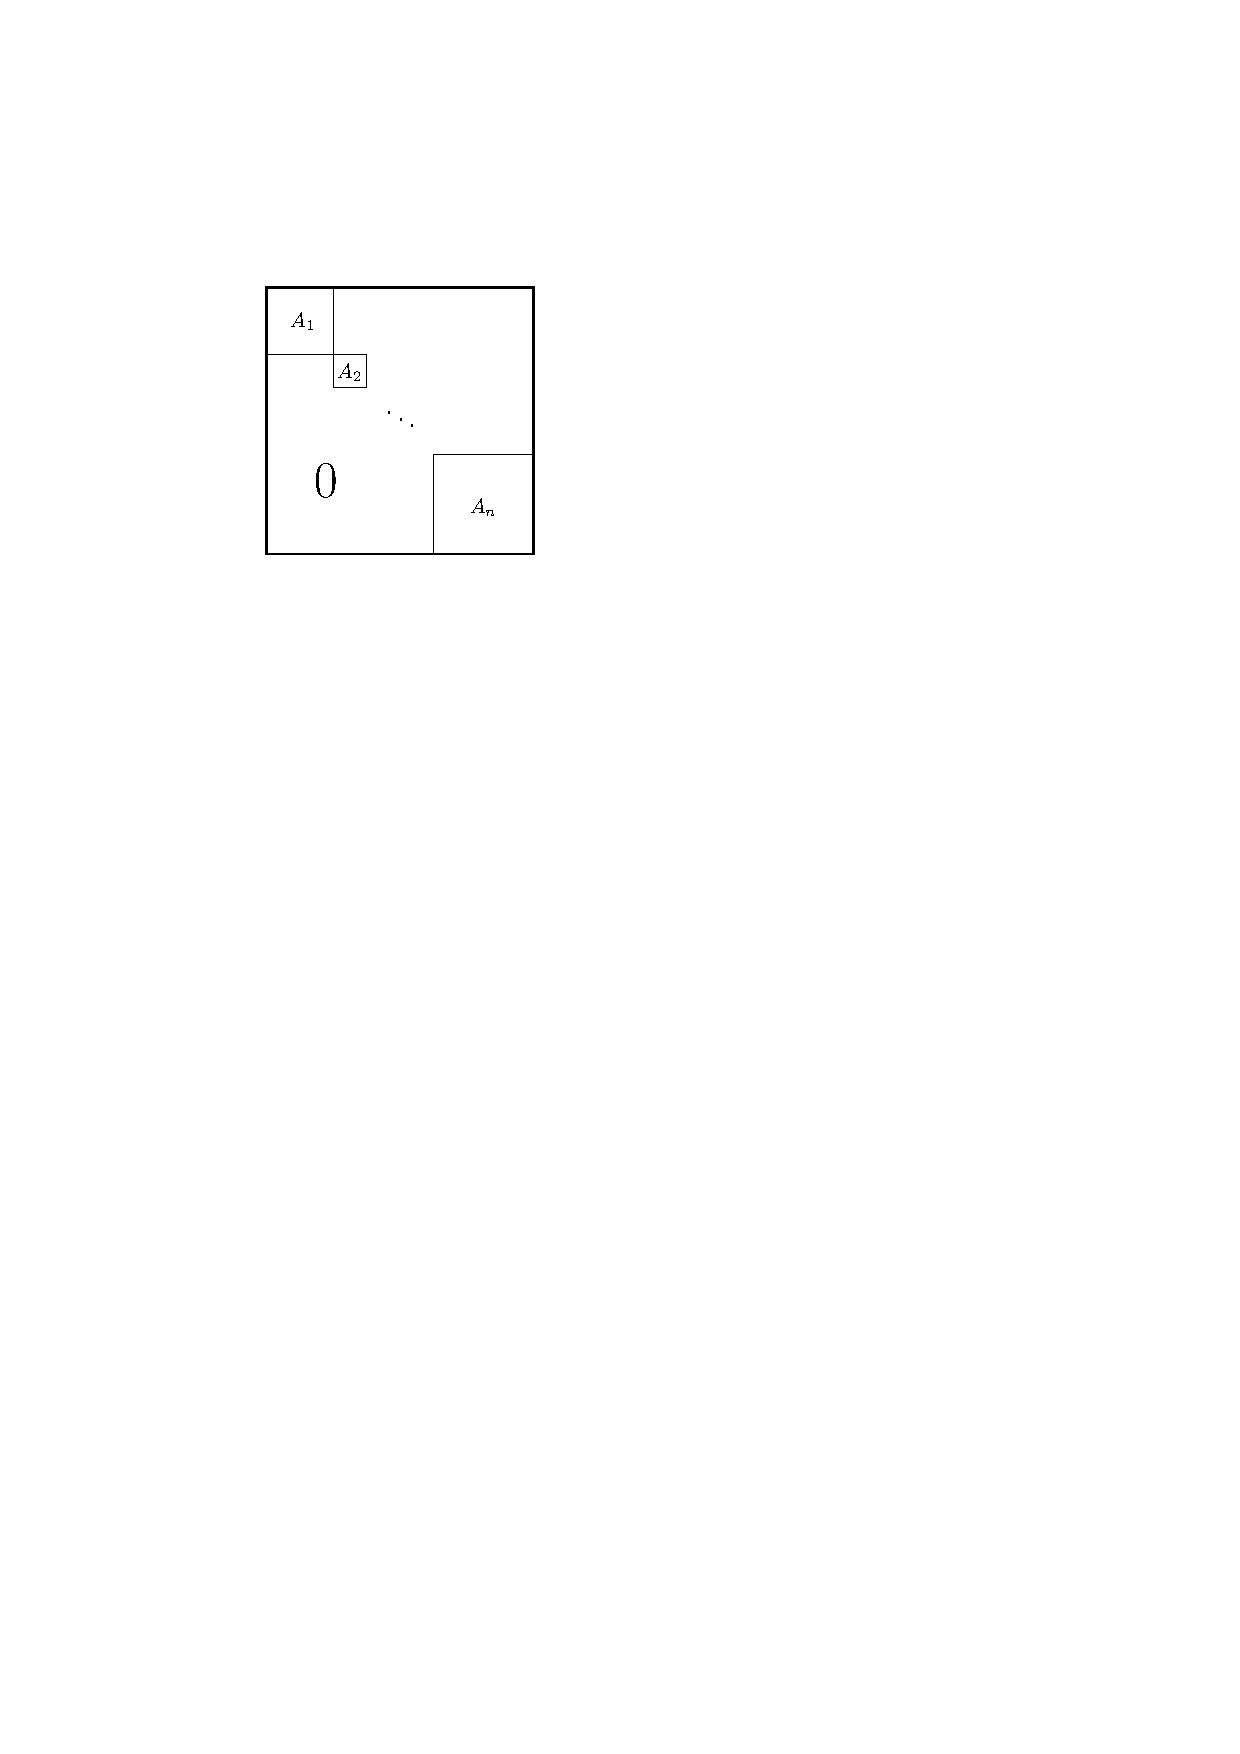
\includegraphics[scale=0.6]{stairsmtx}}~--- ступенчатая 
  матрица.
\end{defn}
\begin{thrm}[Определитель ступенчатой матрицы]\label{thrm:stairsdet}
  \[
    \det A = \det A_1 \dotsm \det A_n
  \]
\end{thrm}
\begin{ittproof}
  По индукции через теорему Лапласа~\ref{thrm:laplacecofactor}
\end{ittproof}

\paragraph{Определитель произведения матриц}
\begin{thrm}\label{thrm:detmult}
  Пусть $A,B \in M_n(K)$. Тогда
  \[
    \det (AB)  = \det A \cdot \det B
  \]
\end{thrm}
\begin{ittproof}
  Докажем, что такие матрицы имеют одинаковый определитель:
  \[
    C = 
    \left(
    \begin{array}[h]{c|c}
      A    & 0 \\
      \hline 
      -E_n & B
    \end{array}
    \right) \quad \text{и} \quad 
    D = 
    \left(
    \begin{array}[h]{c|c}
      AB    & A \\
      \hline 
      0 & -E_n
    \end{array}
    \right)
  \]


\end{ittproof}


\end{document}
